\documentclass{article}

\title{\sc\LARGE CSCA67 Tutorial, Week 5\\
{\Large Oct. 19th-Oct. 23rd, 2015}}
\date{}
\author{\sc Compiled by {\em G. Singh Cadieux}\\[1ex]
\sc Adapted from\\
A. Bretscher, \href{http://www.utsc.utoronto.ca/~bretscher/a67/lectures/w5.pdf}{\em CSCA67 Week 5 Lecture Notes} \&\\
Evans and Rosenthal. \textit{Probability and Statistics: The Science of Uncertainty}.
W. H. Freeman\\
and Company, 2010.}

\usepackage{fullpage}
\usepackage{amsmath,amssymb}
%\usepackage{color}
%\usepackage{multicol}
\usepackage{tikz}
\usepackage{hyperref}

\setlength{\parindent}{0pt}

\begin{document}
\maketitle

\section{\sc Review of week 5's lecture}
\subsection{\em The Birthday Problem}

\textsc{Q: What is the probability that, in a group of $n$ people, at least 2 have the same birthday?}\\[1em]
Let us represent the days of the year by the integers 1, 2, \ldots, 365. Then we choose our sample space $\textsl{S}$ to be \{all possible combinations of $n$ birthdays\}. That is, we include all possible combinations of $n$ days, with repetition (up to $n$ repetitions of the same day, where all $n$ birthdays fall on the same day).\\[1ex]
For example, if $n=3$, we include:
\begin{itemize}
\item all the single days of the year (eg. (1, 1, 1), (2, 2, 2), (3, 3, 3), \ldots), in the case that all 3 birthdays fall on the same day,
\item all combinations of 2 different days of the year (eg. (1, 1, 2), (1, 1, 3), (1, 1, 4), \ldots), in the case that 2 of the birthdays fall on the same day, and
\item all combinations of 3 different days of the year (eg. (1, 2, 3), (1, 2, 4), (1, 2, 5), \ldots), in the case that all 3 birthdays fall on different days
\end{itemize}
Suppose that all birthdays are equally likely. Then, by the classical definition of probability,
\begin{equation*}
P(\{\text{at least 2 people share a birthday}\})=\dfrac{|\{\text{at least 2\ldots}\}|}{|\textsl{S}|}
\end{equation*}
We know from counting principles that
\begin{align*}
|\textsl{S}|& =\text{\# of ways to select the first birthday $\times$ \# of ways to select the second birthday}\\
& \quad\times\ldots\times\text{\# of ways to select the $n$th birthday}\\
& =365\times 365\times\ldots\times 365\\
& =365^n
\end{align*}
and that
\begin{align*}
|\{\text{at least 2\ldots}\}|& =\text{\# of arrangements of $n$ birthdays where 2 people share a birthday}\\
& \quad+\text{\# of arrangements of $n$ birthdays where 3 people share a birthday}\\
& \quad+\ldots+\text{\# of arrangements of $n$ birthdays where $n$ people share a birthday}
\end{align*}
So
\begin{equation*}
P(\{\text{at least 2 people share a birthday}\})=\dfrac{|\{\text{2 people share a birthday}\}|+\ldots+|\{\text{$n$ people share a birthday}\}|}{365^n}
\end{equation*}
%Then we consider that
%\begin{align*}
%\text{\# of arrangements of $n$ birthdays}& \\
%\text{where $r$ people share a birthday}& =\text{\# of ways to select the first unshared birthday}\\
%& \quad\times\text{\# of ways to select the second unshared birthday}\\
%& \quad\times\ldots\times\text{\# of ways to select the $(n-r)$th unshared birthday}\\
%& \quad\times\text{\# of ways to select the $n-r$ people with unshared birthdays}\\
%& \quad\times \text{\# of ways to select the shared birthday}\\
%& =365\times 364\times\ldots\times(365-(n-r)+1)\times \binom{n}{n-r}\times(365-(n-r))
%\end{align*}
%For example, if $n=3$, 
%\begin{align*}
%\text{\# of arr. where 2 people share a birthday}& =\text{\# of ways to select the unshared birthday}\\
%& \quad\times\text{\# of ways to select the 1 person with an unshared birthday}\\
%& \quad\times \text{\# of ways to select the shared birthday}\\
%& =365\times \tbinom{3}{3-2}\times 364\\
%& =398\,580
%\end{align*}
%\textsc{So}
%\begin{align*}
%|\{\text{at least 2\ldots}\}|& =(365\times 364\times\ldots\times(365-(n-2)+1)\times \tbinom{n}{n-2}\times(365-(n-2)))\\
%& \quad+(365\times 364\times\ldots\times(365-(n-3)+1)\times \tbinom{n}{n-3}\times(365-(n-3)))\\
%& \quad+\ldots+(365\times 364\times\ldots\times(365-(n-n)+1)\times \tbinom{n}{n-n}\times(365-(n-n)))\\
%& =\sum\limits_{i=2}^n \left(\binom{n}{n-i}\prod\limits_{j=0}^{n-i}(365-j)\right)
%\end{align*}
%and
%\begin{equation*}
%P(\{\text{at least 2 people share a birthday}\})=\dfrac{\sum\limits_{i=2}^n \left(\binom{n}{n-i}\prod\limits_{j=0}^{n-i}(365-j)\right)}{365^n}
%\end{equation*}
\textsc{However}, this seems very laborious to compute, particularly if $n$ is large.\\
We can instead use the complement rule to determine that
\begin{align*}
P(\{\text{at least 2 people share a birthday}\})& =1-P(\{\overline{\text{at least 2 people share a birthday}}\})\\
& =1-P(\{\text{no shared birthdays}\})\\
& =1-\dfrac{\text{\# of ways to select $n$ unshared birthdays}}{365^n}\\
& =1-\dfrac{365\times 364\times\ldots\times(365-n+1)}{365^n}
\end{align*}
\textsc{Notice} that, if $n>365$, the above calculation produces
\begin{align*}
P(\{\text{at least 2\ldots}\})& =1-\dfrac{365\times(365-1)\times\ldots\times(365-364)\times(365-365)\times\ldots\times(365-n+1)}{365^n}\\
& =1-\dfrac{365\times\ldots\times 0\times\ldots\times(365-n+1)}{365^n}\\
& =1-\dfrac{0}{365^n}\\
& =1-0=1
\end{align*}
Why does this make sense?\\[1ex]
By the pigeonhole principle, if we have $n$ objects to place in fewer than $n$ pigeonholes, at least 1 pigeonhole will contain multiple objects. In this case, if there are more than 365 birthdays to distribute over 365 days, at least 2 birthdays will fall on the same day. Thus, the probability of at least 2 people sharing a birthday is 1, or absolutely certain.\\[1ex]
\textsc{Note} that this counting method counts \textit{ordered} $n$-tuples: for example, where $n=3$, we consider (1, 1, 2) and (1, 2, 1) to be different combinations of birthdays.\\
If we were to instead consider unordered $n$-tuples, we could not use the classical definition of probability, since not all outcomes would be equally likely. For example, where $n=3$, the unordered combination (1, 1, 2) is more likely than the unordered combination (1, 2, 3), since there are more ways in which the former can occur.

\subsection{\em Conditional Probability}
Given two events $A$ and $B$ for an experiment, the {\sc conditional probability} of $A$ given $B$, written $P(A|B)$, represents the fraction of time that $A$ occurs once we \textit{know} that $B$ occurs.\\[1ex]
$P(E)$ represents the fraction of time that an event $E$ occurs. For example, if $P(E)=50\%$ and we conduct 10 trials of our experiment, 5 of those trials will result in $E$.\\
Recall that $A\cap B$ is the event that both $A$ and $B$ occur.\\
Thus, the conditional probability
\begin{equation*}
P(A|B)=\dfrac{P(A\cap B)}{P(B)}\quad\text{with }P(B)>0
\end{equation*}
represents the ratio between the fraction of time that $B$ occurs and the fraction of time that $A\cap B$ occurs.\pagebreak\\
\textsc{Consider} the experiment of tossing two fair coins. Let $A$ be the event that the first coin is heads, and let $B$ be the event that exactly two coins are heads.\\[1ex]
If we let our sample space $\mathcal{S}$ be $\{HH, HT, TH, TT\}$, then this is an equally-likely sample space and we can compute that
\begin{gather*}
P(A)=\dfrac{|A|}{|\mathcal{S}|}=\frac{|\{HH,HT\}|}{|\{HH, HT, TH, TT\}|}=\dfrac{2}{4}\qquad\qquad
P(B)=\dfrac{|B|}{|\mathcal{S}|}=\frac{|\{HH\}|}{|\{HH, HT, TH, TT\}|}=\dfrac{1}{4}\\[1ex]
P(A\cap B)=\dfrac{|A\cap B|}{|\mathcal{S}|}=\frac{|\{HH\}|}{|\{HH, HT, TH, TT\}|}=\dfrac{1}{4}
\end{gather*}
Using the definition above, we can also compute that
\begin{equation*}
P(A|B)=\dfrac{P(A\cap B)}{P(B)}=\dfrac{|A\cap B|/|\mathcal{S}|}{|B|/|\mathcal{S}|}=\dfrac{|A\cap B|}{|B|}=\dfrac{|\{HH\}|}{|\{HH\}|}=1
\end{equation*}
\textsc{Notice} that $P(A\cap B)=\dfrac{|A\cap B|}{|\mathcal{S}|}$ is very similar to $P(A|B)=\dfrac{|A\cap B|}{|B|}$. The difference is that, in the former case, we consider the fraction of time that $A\cap B$ occurs out of \textit{all} possible outcomes, while in the latter case, we consider the fraction of time that $A\cap B$ occurs out of the times that $B$ occurs (ignoring the times that $B$ does \textit{not} occur).\\
Put another way: $P(B|A)$ answers the question, ``if $B$ occurs, what is the probability that $A$ \textit{also} occurs?"\\[1em]
\textsc{Notice also} that, in this example, $P(A|B)>P(A)$. This tells us that $B$ occurring increases the likelihood that $A$ will occur.\\
Intuitively, this makes sense: if both coins are heads ($B$ occurs), then the first coin \textit{must} be heads (event $A$ occurs with probability 1); but if we do not know whether either coin is heads, it is possible for the first coin to be tails (event $A$ occurs with probability $<1$).\\[1ex]
However, if $C$ is the event that exactly two coins are tails, then
\begin{equation*}
P(A|C)=\dfrac{|A\cap C|}{|C|}=\frac{|\emptyset|}{|\{TT\}|}=0
\end{equation*}
Here, $P(A|C)<P(A)$ - that is, $C$ occurring \textit{decreases} the likelihood that $A$ will occur.\\
Again, intuitively, this makes sense: if both coins are tails ($C$ occurs), then the first coin \textit{cannot} be heads (event $A$ occurs with probability 0); but if we do not know whether either coin is heads, it is possible for the first coin to be heads (event $A$ occurs with probability $>0$).\\[1ex]
And if $D$ is the event that the second coin is heads, then
\begin{equation*}
P(A|D)=\dfrac{|A\cap D|}{|D|}=\frac{|\{HH\}|}{|\{TH, TT\}|}=\dfrac{1}{2}
\end{equation*}
Here, $P(A|D)=P(A)$ - that is, $D$ occurring \textit{does not affect} the likelihood that $A$ will occur.

\subsubsection*{\em Independence of Events}
If $P(E|F)=P(E)$ or $P(F|E)=P(F)$ for two events $E$ and $F$, where $P(F)>0$ or $P(E)>0$ respectively, we say that $E$ and $F$ are \textsc{independent}. Intuitively, this means that the occurrence of $E$ does not affect the probability of $F$ occurring, and vice versa.

\subsubsection*{\em Product Rule}
We can reformulate the above definition of conditional probability for two events $A$ and $B$ as:
\begin{equation*}
P(A\cap B)=P(A|B)\cdot P(B)=P(B|A)\cdot P(A)
\end{equation*}
This allows us to compute the probability of $A\cap B$ when we are given the probability of $A$ and the conditional probability of $B$ given $A$, or the probability of $B$ and the conditional probability of $A$ given $B$.\\[1em]
\textsc{Notice} that, if $A$ and $B$ are independent, then
\begin{align*}
P(A\cap B)&=P(A|B)\cdot P(B)=P(A)\cdot P(B)\quad and\\
P(A\cap B)&=P(B|A)\cdot P(A)=P(B)\cdot P(A)
\end{align*}
which is an alternative definition of independence for two events $A$ and $B$.

\subsubsection*{\em Bayes' theorem}
We can also reformulate the above definition of conditional probability for two events $A$ and $B$ as:
\begin{equation*}
\mathbf{P(A|B)}=\dfrac{P(A\cap B)}{P(B)}=\dfrac{P(A\cap B)}{P(B)}\cdot\dfrac{P(A)}{P(A)}=\dfrac{P(A\cap B)}{P(A)}\cdot\dfrac{P(A)}{P(B)}=\mathbf{P(B|A)\cdot\dfrac{P(A)}{P(B)}}\quad\text{with }P(A),\,P(B)>0
\end{equation*}
This allows us to compute the conditional probability of $B$ given $A$ when we are given the probability of $A$, $B$, and the conditional probability of $A$ given $B$.\\[1em]
For example, suppose that the probability of snow is 20\%, and the probability of a traffic accident is 10\%. Suppose further that the conditional probability of an accident, given that it snows, is 40\%.\\[1ex]
{\sc Q: What is the conditional probability that it snows given that there is a traffic accident?}\\[1em]
Using Bayes' theorem with $A=\text{snow}$ and $B=\text{traffic accident}$, we can calculate that
\begin{align*}
P(\text{snow}|\text{traffic accident})&=\dfrac{P(\text{snow})}{P(\text{traffic accident})}\cdot P(\text{traffic accident}|\text{snow})\\
&=\dfrac{0.2\cdot 0.4}{0.1}\\
&=0.8=80\%
\end{align*}

\subsubsection*{\em Law of Total (Conditioned) Probability}
Let $E_1,E_2,\ldots,E_n$ be events that form a partition of the sample space $\mathcal{S}$, each with positive probability. Let $A\subseteq\mathcal{S}$ be any event. Then
\begin{align*}
P(A)&=P(E_1\cap A)+P(E_2\cap A)+\ldots+P(E_n\cap A)\\
&=P(E_1)\cdot P(A|E_1)+P(E_2)\cdot P(A|E_2)+\ldots+P(E_n)\cdot P(A|E_n)\qquad\text{[by the product rule]}\\
&=\sum\limits_{i=1}^nP(E_i)\cdot P(A|E_i)
\end{align*}
Represented as a Venn diagram (with $n=7$):
\begin{center}
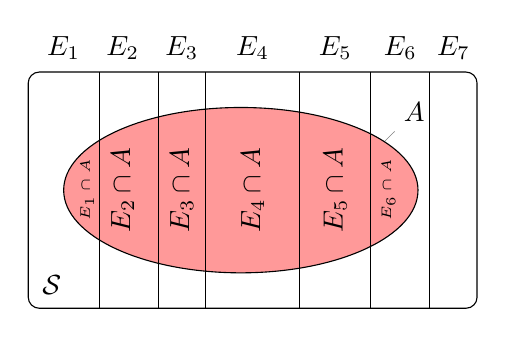
\begin{tikzpicture}[scale=1.5]
\draw[rounded corners] (0,0) rectangle (3.8,2);
\node at (0.2,0.2) {$\mathcal{S}$};
\node[pin=above right:{$A$}] at (2.8,1.2) {};
\draw[fill=red!40] (1.8,1) ellipse [x radius=1.5, y radius=0.7];

\draw (0.6,0) -- (0.6,2);
\node at (0.3,2.2) {$E_1$};
\draw (1.1,0) -- (1.1,2);
\node at (0.8,2.2) {$E_2$};
\draw (1.5,0) -- (1.5,2);
\node at (1.3,2.2) {$E_3$};
\draw (2.3,0) -- (2.3,2);
\node at (1.9,2.2) {$E_4$};
\draw (2.9,0) -- (2.9,2);
\node at (2.6,2.2) {$E_5$};
\draw (3.4,0) -- (3.4,2);
\node at (3.15,2.2) {$E_6$};
\node at (3.6,2.2) {$E_7$};

\node[rotate=90] at (0.5,1) {\tiny $E_1\cap A$};
\node[rotate=90] at (0.8,1) {$E_2\cap A$};
\node[rotate=90] at (1.3,1) {$E_3\cap A$};
\node[rotate=90] at (1.9,1) {$E_4\cap A$};
\node[rotate=90] at (2.6,1) {$E_5\cap A$};
\node[rotate=90] at (3.05,1) {\tiny $E_6\cap A$};
\end{tikzpicture}
\end{center}
For example, suppose that a class contains 60\% girls and 40\% boys. Suppose that 30\% of the girls have long hair and 20\% of the boys have long hair.\\[1ex]
\textsc{Q: If a student is chosen randomly from the class, what is the probability that he or she has long hair?}\\[1em]
Let $\mathcal{S}$ be the class of students.\\
If we let $E_1$ be the event that we choose a girl, and $E_2$ be the event that we choose a boy, then $E_1$ and $E_2$ partition $\mathcal{S}$ (since either $E_1$ or $E_2$ must occur, but $E_1$ and $E_2$ cannot both occur).\\[1ex]
Using the law of total (conditioned) probability, we can calculate that
\begin{align*}
P(\text{long hair})&=P(\text{girl})\cdot P(\text{long hair}|\text{girl})+P(\text{boy})\cdot P(\text{long hair}|\text{boy})\\
&=60\%\cdot 30\%+40\%\cdot 20\%\\
&=26\%
\end{align*}

\section{\sc Probability problems}

\subsection*{{\normalsize Suppose that we roll four fair six-sided dice.}\\
Q: {\em What is the conditional probability that the first die shows 2, conditional on the event that exactly three dice show 2?}}

Let our (equally-likely) sample space $\mathcal{S}$ be $\{(1,1,1,1),(1,1,1,2),\ldots,(6,6,6,6)\}$.\\
Let $A$ be the event that exactly three dice show 2, and let $B$ be the event that the first die shows 2.\\
Then we know from the definition of conditional probability that
\begin{equation*}
P(B|A)=\dfrac{P(A\cap B)}{P(A)}=\dfrac{|A\cap B|/|\mathcal{S}|}{|A|/|\mathcal{S}|}=\dfrac{|A\cap B|}{|A|}
\end{equation*}
$A\cap B$ is the event that exactly three dice show 2, including the first die.\\
So $A=\{(2,2,2,1),(2,2,2,3),\ldots,(6,2,2,2)\}$, and of this,
$A\cap B=\{(2,2,2,1),(2,2,2,3),\ldots,(2,6,2,2)\}$.\\[1ex]
We calculate that $|A|=(4\text{ ways to choose the die not showing 2})\times(5\text{ ways to choose its value})=20$ and\\
$|A\cap B|=(3\text{ ways to choose the die not showing 2})\times(5\text{ ways to choose its value})=15$. So
\begin{equation*}
P(B|A)=\dfrac{15}{20}=\dfrac{3}{4}
\end{equation*}

%\subsubsection*{b) {\em at least three dice show 2?}}
%
%Using the same sample space $\mathcal{S}$ as in (a), we let $A$ be the event that at least three dice show 2, and let $B$ be the event that the first die shows 2.\\
%Again, we know that
%\begin{equation*}
%P(B|A)=\dfrac{P(A\cap B)}{P(A)}=\dfrac{|A\cap B|/|\mathcal{S}|}{|A|/|\mathcal{S}|}=\dfrac{|A\cap B|}{|A|}
%\end{equation*}
%Here, $A=\{\text{3 dice show 2},\,\text{4 dice show 2}\}=\{(2,2,2,1),(2,2,2,3),\ldots,(6,2,2,2),(2,2,2,2)\}$, and of this, $A\cap B=\{(2,2,2,1),(2,2,2,3),\ldots,(2,6,2,2),(2,2,2,2)\}$.\\[1ex]
%We can see that we have $A$ and $A\cap B$ almost identical to those in (a), but each with the additional outcome $(2,2,2,2)$. So\\
%\begin{equation*}
%P(B|A)=\dfrac{15+1}{20+1}=\dfrac{16}{21}
%\end{equation*}

\subsection*{{\normalsize Suppose we deal five cards from an ordinary 52-card deck.}\\
Q: {\em What is the conditional probability that all five cards are spades, given that at least four of them are spades?}}
Let our (equally-likely) sample space $\mathcal{S}$ be all possible combinations of 5 cards. Let $A$ be the event that all five cards are spades, and let $B$ be the event that at least four of the cards are spades.\\
Then we can use the definition of conditional probability to calculate
\begin{align*}
P(A|B)&=\dfrac{P(A\cap B)}{P(B)}=\dfrac{|A\cap B|/|\mathcal{S}|}{|B|/|\mathcal{S}|}=\dfrac{|A\cap B|}{|B|}\\
&=\dfrac{|\{\text{5 spades and at least 4 spades}\}|}{|\{\text{at least 4 spades}\}|}=\dfrac{|\{\text{5 spades}\}|}{|\{\text{at least 4 spades}\}|}\\
&=\dbinom{13\text{ spades}}{5\text{ spades}}\Big/\Big({\dbinom{13\text{ spades}}{4\text{ spades}}\cdot\binom{39\text{ non-spades}}{1\text{ non-spade}}+\binom{13\text{ spades}}{5\text{ spades}}}\Big)\\
&=\dfrac{1287}{29172}\approx 0.044
\end{align*}

\subsection*{{\normalsize Suppose that we have one jar with 3 red and 2 blue balls, and a second jar with 4 red and 7 blue balls.}\\
Q: {\em If we pick one of the jars at random, and then pick one of the balls in that jar at random, what is the probability that}}
\subsubsection*{a) {\em the second jar is picked and then a blue ball is picked?}}

Let $A$ be the event that the second jar is picked, and let $B$ be the event that a blue ball is picked.\\
Then we can use the product rule to calculate
\begin{align*}
P(A\cap B)&=P(A)\cdot P(B|A)\\
&=\dfrac{1}{2}\cdot\dfrac{7\text{ blue balls}}{11\text{ total balls}}\\
&=\dfrac{7}{22}
\end{align*}

\subsubsection*{b) {\em a blue ball is picked?}}
Let $B$ be the event that a blue ball is picked. Let $A_1$ be the event that the first jar is picked, and let $A_2$ be the event that the second jar is picked.\\
Then we can use the law of total (conditioned) probability to calculate
\begin{align*}
P(B)&=P(E_1)\cdot P(A|E_1)+P(E_2)\cdot P(A|E_2)P(A_1)\cdot P(B|A_1)+P(A_2)\cdot P(B|A_2)\\
&=\dfrac{1}{2}\cdot\dfrac{2\text{ blue balls}}{5\text{ total balls}}+\dfrac{1}{2}\cdot\dfrac{7\text{ blue balls}}{11\text{ total balls}}\\
&=0.5\overline{18}
\end{align*}

\subsubsection*{c) {\em the second jar was picked, given that we picked a blue ball?}}
Again, let $A$ be the event that the second jar is picked, and let $B$ be the event that a blue ball is picked. Since we know $P(A),P(B),P(B|A)$, we can use Bayes' theorem to calculate
\begin{align*}
P(A|B)&=\dfrac{P(A)}{P(B)}\cdot P(B|A)\\
&=\dfrac{1/2}{0.5\overline{18}}\cdot\dfrac{7\text{ blue balls}}{11\text{ total balls}}\\
&\approx 0.614
\end{align*}

\subsection*{{\normalsize Suppose that we roll two fair six-sided dice.\\
Let $A$ be the event that the two dice show the same value.\\
Let $B$ be the event that the sum of the two dice is equal to 12.\\\
Let $C$ be the event that the first die shows 4.\\
Let $D$ be the event that the second die shows 4.}\\
Q: {\em Which events are independent of one another?}}
Let us choose $\{(1,1),(1,2),\ldots,(6,6)\}$ as our (equally-likely) sample space $\mathcal{S}$. Then
\begin{align*}
P(A)&=\dfrac{|A|}{|\mathcal{S}|}=\dfrac{|\{(1,1),(2,2),\ldots,(6,6)\}|}{6^2}=\dfrac{6}{6^2}=\dfrac{1}{6}&P(C)&=\dfrac{|C|}{|\mathcal{S}|}=\dfrac{|\{(4,1),(4,2),\ldots,(4,6)\}|}{6^2}=\dfrac{6}{6^2}=\dfrac{1}{6}\\[1ex]
P(B)&=\dfrac{|B|}{|\mathcal{S}|}=\dfrac{|\{(6,6)\}|}{6^2}=\dfrac{1}{6^2}&P(D)&=\dfrac{|D|}{|\mathcal{S}|}=\dfrac{|\{(1,4),(2,4),\ldots,(6,4)\}|}{6^2}=\dfrac{6}{6^2}=\dfrac{1}{6}
\end{align*}
We know that two events $E$ and $F$ are independent if $P(E|F)=P(E)$ or if $P(F|E)=P(F)$, with $P(E),\,P(F)>0$. And we know from the definition of conditional probability that $P(E|F)=\frac{P(E\cap F)}{P(F)}$. So
\begin{align*}
P(A|B)&=\dfrac{P(A\cap B)}{P(B)}=\dfrac{|A\cap B|/|\mathcal{S}|}{P(B)}=\dfrac{|\{(6,6)\}|/6^2}{1/6^2}=\dfrac{1/6^2}{1/6^2}=1\neq P(A)&&\Rightarrow\text{$A$ and $B$ are not independent}\\[1ex]
P(A|C)&=\dfrac{P(A\cap C)}{P(C)}=\dfrac{|A\cap C|/|\mathcal{S}|}{P(C)}=\dfrac{|\{(4,4)\}|/6^2}{1/6}=\dfrac{1/6^2}{1/6}=\dfrac{1}{6}=P(A)&&\Rightarrow\text{$A$ and $C$ are independent}\\[1ex]
P(A|D)&=\dfrac{P(A\cap D)}{P(D)}=\dfrac{|A\cap D|/|\mathcal{S}|}{P(D)}=\dfrac{|\{(4,4)\}|/6^2}{1/6}=\dfrac{1/6^2}{1/6}=\dfrac{1}{6}=P(A)&&\Rightarrow\text{$A$ and $D$ are independent}\\[1ex]
P(B|C)&=\dfrac{P(B\cap C)}{P(C)}=\dfrac{|B\cap C|/|\mathcal{S}|}{P(C)}=\dfrac{|\emptyset|/6^2}{1/6}=\dfrac{0}{1/6}=0\neq P(B)&&\Rightarrow\text{$B$ and $C$ are not independent}\\[1ex]
P(B|D)&=\dfrac{P(B\cap D)}{P(D)}=\dfrac{|B\cap D|/|\mathcal{S}|}{P(D)}=\dfrac{|\emptyset|/6^2}{1/6}=\dfrac{0}{1/6}=0\neq P(B)&&\Rightarrow\text{$B$ and $C$ are not independent}\\[1ex]
P(C|D)&=\dfrac{P(C\cap D)}{P(D)}=\dfrac{|C\cap D|/|\mathcal{S}|}{P(D)}=\dfrac{|\{(4,4)\}|/6^2}{1/6}=\dfrac{1/6^2}{1/6}=\dfrac{1}{6}=P(C)&&\Rightarrow\text{$C$ and $D$ are independent}
\end{align*}



\subsection*{Monty Hall Problem}
\textsc{See} \href{https://www.youtube.com/watch?v=mhlc7peGlGg\&authuser=0}{\em The Monty Hall Problem} \textsc{or} \href{https://www.youtube.com/watch?v=7u6kFlWZOWg\&authuser=0}{\em Monty Hall Problem for Dummies - Numberphile}.

\section{\sc Additional practice problems}
{\bf Q: What is the probability of having the same birthday as your mother?}\\[1em]
{\bf Q: Approximately how many people in the world have the same birthday as their mother?}\\[1em]
{\bf Q: Approximately how many people in the world have the same birthday as their mother, father, \textit{and} spouse?}\\[1em]
Suppose we deal five cards from an ordinary 52-card deck.\\
{\bf Q: What is the conditional probability that the hand contains all four aces, given that the hand contains at least four aces?}\\[1ex]
{\bf Q: What is the conditional probability that the hand contains no pairs, given that it contains no spades?}\\[1em]
Suppose we roll a fair six-sided die and then flip a number of fair coins equal to the number showing on the die (eg. if the die shows 4, then we flip 4 coins).\\
{\bf Q: What is the probability that the number of heads equals 3?}\\[1ex]
{\bf Q: Conditional on knowing that the number of heads equals 3, what is the probability that the die showed the number 5?}\\[1em]
Suppose a baseball pitcher throws fastballs 80\% of the time and curveballs 20\% of the time. Suppose a batter hits a home run on 8\% of all fastball pitches, and on 5\% of all curveball pitches.\\
{\bf Q: What is the probability that this batter will hit a home run on this pitcher's next pitch?}


\end{document}